% Versión en español, autocontenida (conceptos explicados al usarse) y acotada.
% Compilar con pdfLaTeX (Overleaf). Las figuras viven en figures/.
\documentclass[11pt]{article}
\usepackage[a4paper,margin=2.3cm]{geometry}
\usepackage{iftex}
\ifPDFTeX
  \usepackage[utf8]{inputenc}
  \usepackage[T1]{fontenc}
\else
  \usepackage{fontspec}
\fi
\usepackage[spanish,es-tabla,shorthands=off]{babel}
\usepackage{graphicx}
\usepackage{amsmath}
\usepackage{booktabs}
\usepackage{caption}
\usepackage[hidelinks]{hyperref}
\graphicspath{{figures/}}
\captionsetup{font=small}

\title{\vspace{-1.2cm}Un retardo distribuido de acumulación en el ciclo ganancias--inversión:\\
calibración inversa diferenciable y límites de identificabilidad}
\author{Juan I. Tollo}
\date{\today}

\begin{document}
\maketitle
\vspace{-0.7cm}

\begin{abstract}
\noindent
Estudiamos el ciclo ganancias--inversión de la economía de EE.UU.\ (datos trimestrales,
1948--2026) desde la hipótesis de \emph{sobreacumulación}: la inversión pasada deprime la
rentabilidad presente con un retardo. Documentamos un co-movimiento contemporáneo dominante
junto con un feedback negativo centrado en $\sim$1 año, que se acumula antes de las recesiones.
Los osciladores depredador--presa de fase fija
(Lotka--Volterra, FitzHugh--Nagumo) no pueden reproducir esa forma. Proponemos en cambio un
modelo físico de \emph{cadena de acumulación} ---una ecuación diferencial con retardo
distribuido--- y lo calibramos resolviendo un problema inverso diferenciable (una red neuronal
informada por la física, PINN, con \emph{features} de Fourier). El método recupera el retardo
limpiamente en datos sintéticos (error del $8{,}9\%$) y estima $\approx$1 año en los datos
reales; la estimación es estable a la transformación de la serie y a excluir cada crisis. El
resultado central es de \emph{identificabilidad}: el \emph{centro} del retardo se identifica de
forma robusta, pero su \emph{dispersión} no, y el feedback es observacionalmente equivalente a
un modelo lineal $\mathrm{VAR}(p\!\ge\!4)$ al nivel de la autocovarianza de segundo orden.
\end{abstract}

\section{Introducción}

\paragraph{La hipótesis económica.} Las ganancias y la inversión forman un ciclo endógeno: las
ganancias altas estimulan la inversión, pero esa misma inversión, al acumularse, erosiona las
ganancias posteriores. Tapia (2023, pp.~183--186) documenta esta estructura bidireccional sobre
datos trimestrales de EE.UU.: las ganancias preceden a la inversión en la misma dirección, y la
inversión pasada tiene un efecto rezagado \emph{negativo} sobre las ganancias. La formaliza como
``un modelo de tipo depredador--presa'' con las ganancias como presa y la inversión como
predador, y advierte que esta segunda dirección (inversión\,$\to$\,ganancias) es la más débil:
significativa en datos anuales pero no en los trimestrales. Leer ese feedback negativo como
\emph{sobreacumulación} ---la inversión que, al acumularse en capacidad instalada, presiona a la
baja la rentabilidad, ``una crisis por sobreacumulación, o sobreinversión'', no por
subacumulación--- es la contribución de Astarita (2012) a la teoría de las crisis. El antecedente formal de estos
osciladores es la dinámica de Lotka--Volterra (LV), usada en macrodinámica y
estimada para el ciclo de ganancias por Goldstein (1999). En un sistema LV, las dos variables
oscilan con un \emph{desfase fijo de $90^\circ$}: el predador sigue a la presa con un cuarto de
ciclo de atraso, siempre, por construcción.

\paragraph{Nuestra pregunta.} Planteamos una pregunta más acotada y mecanística: ¿el feedback
de la inversión hacia las ganancias es un antagonismo \emph{instantáneo} (como imponen esos
osciladores), o uno \emph{retardado}, cuyo tiempo característico refleja la
\emph{acumulación} de la inversión pasada en capacidad instalada? Encontramos lo segundo. La firma empírica es un
co-movimiento contemporáneo más un feedback negativo concentrado alrededor de un año: una
forma que ningún oscilador de fase fija puede generar, pero que un sistema con retardo
distribuido sí. La contribución es descriptiva y metodológica: una estimación del retardo de
acumulación robusta y estable, recuperada por un método inverso diferenciable donde la
calibración clásica falla, junto con una caracterización explícita de \emph{lo que no puede
identificarse} con estos datos.

\section{Datos y métodos}

\paragraph{Datos.} Series trimestrales de EE.UU.: ganancias corporativas y la inversión
privada bruta (FRED, 1948--2026, $n=313$). Trabajamos con tasas de crecimiento
\emph{log trimestre a trimestre} ($x_t=\log Y_t-\log Y_{t-1}$): verificamos que la transformación
interanual habitual (``YoY'', el cambio respecto del mismo trimestre del año anterior)
\emph{inyecta} estructura espuria de orden 4 ---exactamente en el rezago de interés--- e infla
la magnitud aparente del feedback en un factor $\sim$2, por ser una diferencia a 4 trimestres.

\paragraph{Herramientas descriptivas.} Usamos dos. (i) La \emph{función de correlación
cruzada} (CCF), $\rho(k)=\mathrm{corr}(\text{ganancias}_t,\text{inversión}_{t+k})$: un valor
negativo en $k=-4$ significa que la inversión de hace 4 trimestres se asocia con ganancias
\emph{menores} hoy. (ii) Un \emph{estudio de evento}: se alinean las doce recesiones del NBER
en una misma ventana y se promedia, para ver el patrón típico sin que ningún episodio domine.

\paragraph{El modelo físico.} Modelamos la acumulación como una \emph{cadena}: la inversión
atraviesa $n$ etapas antes de deprimir las ganancias. Por el ``truco de la cadena lineal''
(un resultado estándar de ecuaciones con retardo), esto equivale a que el retardo siga una
distribución Gamma de media $\mu$:
\begin{equation}
\dot P = c\,I - d\,P - k\,m,\qquad
\dot I = a\,P - b\,I,\qquad
m(t)=\textstyle\sum_j w_j(\mu)\,I(t-j),
\end{equation}
donde $P$ son las ganancias, $I$ la inversión, $m$ la \emph{inversión acumulada} (un promedio
ponderado de la inversión pasada, con pesos $w(\mu)$ dados por el núcleo Gamma) y $\mu$ es el
\emph{retardo de acumulación}, el parámetro que queremos estimar. El término $-k\,m$ es la
sobreacumulación: la inversión que se acumuló hace $\sim\mu$ trimestres deprime las ganancias
de hoy con intensidad $k$.

\paragraph{El problema inverso y su solución diferenciable.} Estimar $(a,b,c,d,k,\mu)$ a
partir de las series es un \emph{problema inverso}: conocemos la salida (los datos) y buscamos
los parámetros de la ecuación que la generó. Lo resolvemos con una \emph{red neuronal
informada por la física} (PINN; Raissi et al., 2019): una red $t\mapsto[P,I]$ que aproxima
las trayectorias, entrenada con dos términos de pérdida ---uno de ajuste a los datos y otro
que penaliza violar la ecuación diferencial--- optimizando \emph{a la vez} los pesos de la red
y los parámetros físicos ($\mathcal L=\mathcal L_{\text{datos}}+\mathcal L_{\text{física}}$).
Sobre ventanas largas, una red estándar sufre \emph{sesgo espectral} (aprende solo las bajas
frecuencias y el retardo queda sin anclar); lo corregimos con \emph{features de Fourier}
---senos y cosenos de varias frecuencias en lugar del tiempo crudo---, que le permiten
representar las oscilaciones de la serie. Validamos primero en datos \emph{sintéticos}
(generados por el modelo con un retardo conocido): si no recupera un retardo que sabemos
verdadero, no es creíble en datos reales.

\paragraph{Controles de identificabilidad.} \emph{Identificable} significa que los datos
bastan para fijar un parámetro; si distintos valores ajustan igual de bien, no lo está. Lo
evaluamos con: (i) un \emph{perfil de verosimilitud} en $\mu$ (barrerlo fijándolo y reajustando
el resto: si la curva de ajuste es plana, $\mu$ no se identifica); (ii) \emph{leave-one-crisis-out}
(re-estimar excluyendo cada crisis); (iii) un \emph{placebo} (repetir en ventanas sin crisis:
si el patrón aparece igual, no es firma de las crisis); y (iv) la CCF teórica de un
$\mathrm{VAR}(p)$ ---modelo lineal donde cada variable depende de los últimos $p$ rezagos---
vía la ecuación de Lyapunov, para ver si un modelo lineal sin mecanismo ya reproduce el patrón.

\section{Resultados}

\paragraph{El patrón: un feedback retardado, no un antagonismo instantáneo.}
La CCF \emph{oscila} en lugar de decaer: un pico contemporáneo dominante
($\rho(0)\approx+0{,}6$) y un valle negativo (el mínimo de la CCF) en los rezagos 4--5 trimestres
($\approx-0{,}3$), que vuelve a cero hacia el rezago 6 (Fig.~\ref{fig:ccf}). Un
estudio de evento sobre las doce recesiones NBER (alineadas en el valle de la inversión)
confirma el patrón: las ganancias giran primero y la brecha inversión--ganancias se acumula
$\sim$1--1,5 años antes del valle ---el \emph{buildup} de sobreacumulación que precede a las
recesiones. El desfase efectivo es cercano al co-movimiento ($\sim$10$^\circ$), no los
$90^\circ$ de LV/FN; los osciladores de fase fija quedan refutados: su CCF es un coseno
rígido, no un pulso contemporáneo más un valle negativo retardado.

\begin{figure}[t]
\centering
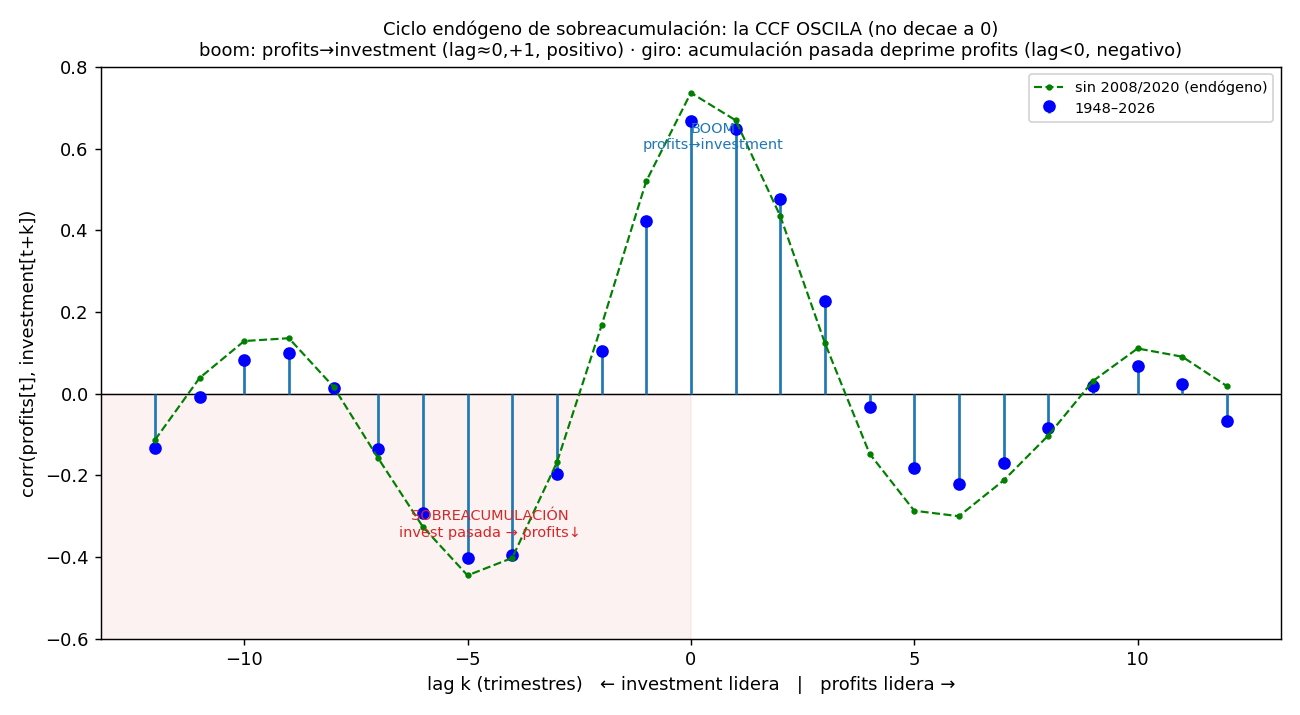
\includegraphics[width=0.58\linewidth]{p7_overaccumulation.png}
\caption{Correlación cruzada ganancias$\leftrightarrow$inversión. La función oscila: fuerte
co-movimiento contemporáneo y un feedback negativo retardado (la inversión acumulada
$\sim$1 año antes deprime las ganancias actuales). Robusto a excluir 2008/2020.}
\label{fig:ccf}
\end{figure}


\paragraph{El retardo de acumulación se identifica y es estable.}
La evidencia central del retardo no es un único método sino la \emph{convergencia} de cuatro
estimadores clásicos en $\approx$4 trimestres: el núcleo empírico, la regresión de rezagos
distribuidos, un $\mathrm{VAR}(p\!\ge\!4)$ y una estimación jerárquica agrupada
($\mu\approx4{,}7$--$4{,}9$). Esa estimación es estable entre transformaciones de diferencia
(log trimestre a trimestre) y al \emph{leave-one-crisis-out} (rango de $0{,}62$ trimestres), de modo
que no depende de ningún episodio. El inverso diferenciable (PINN) aporta una calibración
\emph{física} del mismo retardo: validado en datos sintéticos recupera un retardo conocido
con $8{,}9\%$ de error ($4{,}0\to4{,}36$ trimestres). En datos reales estima $3{,}90$
trimestres $=0{,}98$ años, coincidente con los métodos clásicos; pero advertimos que su ajuste
casi perfecto a la serie ($R^2\approx1$) refleja la \emph{interpolación de la red sustituta}
($\approx$2160 pesos para $\approx$290 valores objetivo), no una validación del modelo de
acumulación (App.~\ref{app:pinn}). El PINN debe leerse, por tanto, como una demostración de
calibración diferenciable \emph{corroborada} por los métodos clásicos, no como la fuente del
retardo. Las otras variantes del inverso (single-shooting, estados latentes libres) colapsan el
retardo o lo sesgan $\sim$55\%; solo la formulación bien puesta ---convolución con el núcleo
Gamma más features de Fourier--- funciona (Apéndice~\ref{app:pinn}).

\paragraph{Lo que no puede identificarse.}
El feedback explica solo $\sim$3\% de la varianza del crecimiento de las ganancias (contra
$\sim$35\% del co-movimiento contemporáneo). De esa debilidad se siguen cuatro límites:
\begin{itemize}
\item \textbf{La dispersión del retardo no es identificable:} el perfil de verosimilitud en el
ancho de la distribución es plano; los datos no distinguen un retardo genuinamente
\emph{distribuido} de un retardo \emph{puntual}.
\item \textbf{El patrón no es específico de las crisis:} el placebo sobre ventanas sin crisis
encuentra el valle negativo con la misma frecuencia fuera de ellas ($p=0{,}34$). El mecanismo
es \emph{estructural y permanente}, no una firma del giro del ciclo.
\item \textbf{Equivalencia observacional con un modelo lineal:} la CCF teórica de un
$\mathrm{VAR}(p\!\ge\!4)$ ajustado reproduce el valle negativo desde sus coeficientes
solamente (Fig.~\ref{fig:var}). El modelo de acumulación es una \emph{reparametrización
interpretable} de ese contenido lineal, no un mecanismo separable de él con estos datos.
\item \textbf{El $k$ del PINN no es una atribución directa:} una descomposición OLS del
término de sobreacumulación $-k\,m$ sobre los datos reales da $\beta_m\approx+0{,}02$
($t\approx0{,}15$, no significativa; signo \emph{contrario} al esperado) con $\Delta R^2\approx0$,
porque la inversión acumulada $m$ es colineal con la
inversión contemporánea $I$. El $k\approx0{,}42$ que reporta el PINN proviene de su red
sustituta sobre-flexible ajustando una penalización casi plana, no de un canal de acumulación
separable del co-movimiento contemporáneo.
\end{itemize}

\begin{figure}[t]
\centering
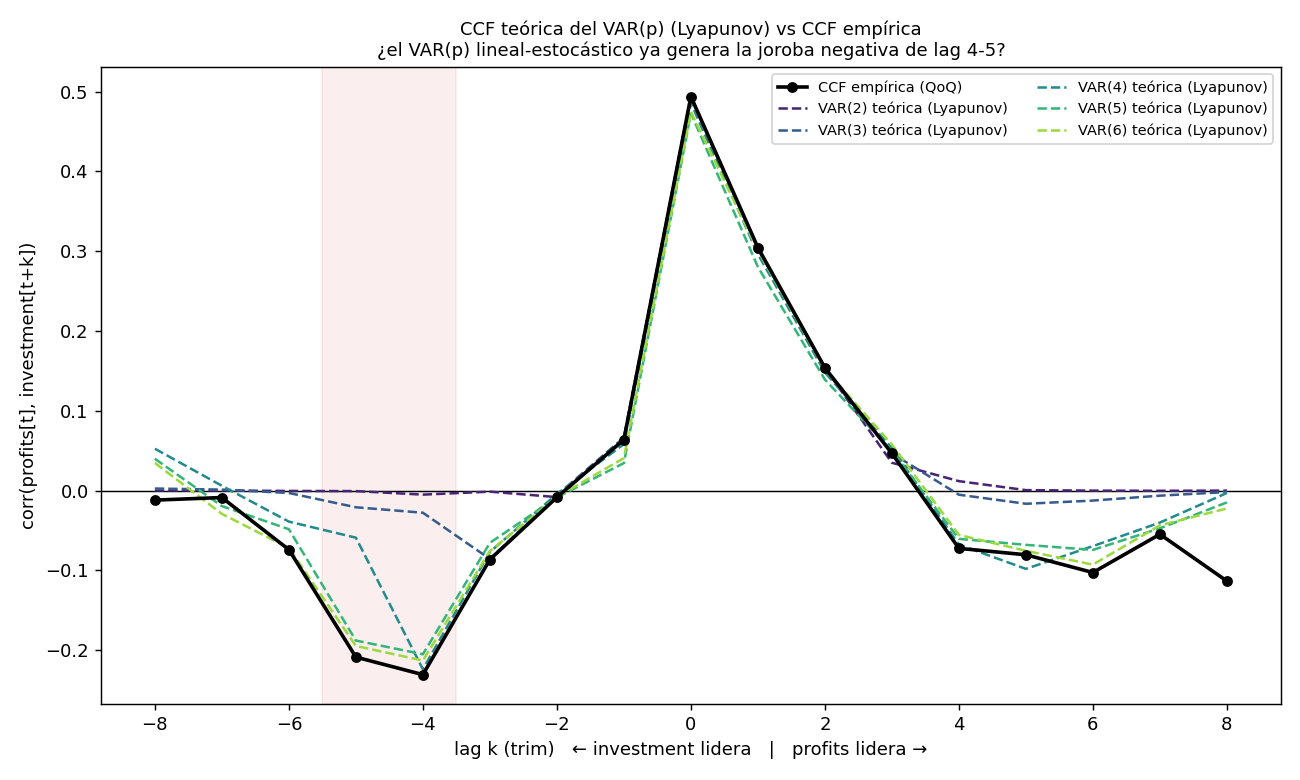
\includegraphics[width=0.52\linewidth]{p12_var_lyapunov_ccf.png}
\caption{CCF teórica de un $\mathrm{VAR}(p)$ ajustado (vía Lyapunov) contra la CCF empírica.
Para $p\ge4$ el modelo lineal ya reproduce el valle negativo de los rezagos 4--5 desde sus
coeficientes: equivalencia observacional con el núcleo de retardo distribuido.}
\label{fig:var}
\end{figure}

\section{Discusión y conclusiones}

El cuadro sustantivo es consistente y honesto. \emph{Existe} un feedback de sobreacumulación
con un retardo de acumulación de alrededor de un año ---estructural antes que específico de las
crisis, ya que el placebo encuentra el valle negativo con igual frecuencia fuera de ellas--- y
lo recuperamos con un modelo físico diferenciable donde la
inversión clásica falla. Dos límites acotan la afirmación. Primero, el contenido económico ---un feedback de sobreacumulación con las ganancias cediendo
antes de las recesiones--- pertenece a la tradición previa (Astarita, 2012; Tapia, 2023);
nuestro aporte es el modelo y el método inverso, no el fenómeno. Segundo, con nueve
crisis de posguerra utilizables y una señal del $\sim$3\% de la varianza, los datos no pueden
separar un retardo genuinamente distribuido de uno puntual, ni el mecanismo de acumulación de
un VAR lineal de memoria larga.

\textbf{Conclusión.} El feedback de sobreacumulación ganancias--inversión queda bien descripto
por un retardo distribuido de acumulación centrado en $\sim$1 año, recuperado por un inverso
diferenciable que supera el sesgo espectral y el mal condicionamiento de la calibración
clásica. El resultado robusto y transferible es la \emph{ubicación de la frontera de
identificabilidad}: el centro del retardo es recuperable y estable; su dispersión, y su
separación de un modelo lineal, no lo son ---una frontera fijada por la fuerza de la señal y
el número de episodios, no por el ajuste fino. Cruzarla requiere datos nuevos, no una
reparametrización.

\section*{Agradecimientos}
El autor utilizó Claude (Anthropic) como asistente para redacción, figuras y código de los
experimentos. Todos los resultados, ecuaciones y conclusiones fueron verificados por el autor,
que asume la responsabilidad por el contenido.

\section*{Datos y software}
Los datos son series públicas de FRED: ganancias corporativas (\texttt{A053RC1Q027SBEA}),
inversión privada bruta (\texttt{GPDI}) y recesiones del NBER (\texttt{USREC}), con un snapshot
versionado para reproducir sin re-descargar. El código (Python~3.12 para el análisis empírico;
Julia con \texttt{Lux.jl}, \texttt{DifferentialEquations.jl} y \texttt{Zygote.jl} para los PINN)
está en \url{https://github.com/JuaniTollo/-flight-to-quality}, con entornos fijados
(\texttt{uv.lock}, \texttt{Manifest.toml}). Series FRED de dominio público; librerías de código
abierto (MIT/BSD).

\appendix

\section{Variantes del PINN inverso}
\label{app:pinn}
El retardo solo es recuperable cuando la red sustituta puede representar la serie y los
parámetros están bien puestos. La Tabla~\ref{tab:pinn} compara cuatro variantes sobre datos
sintéticos (retardo verdadero: 4 trimestres) y sobre la ventana real. Una red estándar sobre
la ventana larga sufre sesgo espectral y el retardo colapsa; el agrupamiento por crisis
arregla el ajuste ($\bar R^2=0{,}86$) pero no el retardo; solo las features de Fourier
recuperan el retardo limpiamente ($8{,}9\%$ de error sintético, $0{,}98$ años en datos
reales). \textbf{Una advertencia sobre el $R^2$ en datos reales.} El $R^2\approx1$ de la fila
real \emph{no} indica que el modelo ajuste: la red sustituta tiene $\approx$2160 pesos para
$\approx$290 valores objetivo y una base de Fourier hasta la frecuencia de Nyquist, de modo que
interpola cualquier serie; el $R^2$ mide esa interpolación, no que la ODE se cumpla. La métrica
honesta es el \emph{residuo físico}, no el $R^2$; por eso el retardo se respalda en la
recuperación sintética y en los métodos no-PINN.

\begin{table}[h]\centering\small
\begin{tabular}{@{}llll@{}}
\toprule
Variante & Sintético (verdadero $4$t) & Retardo real & Veredicto \\
\midrule
Single-shooting / convolución & $1{,}86$t ($54\%$ err) & colapsa a $0{,}23$t, no físico & falla \\
Agrupado por crisis & $1{,}64$t ($59\%$ err) & $0{,}84$t ($\bar R^2\!=\!0{,}86$) & ajusta, retardo colapsa \\
Perfil de verosimilitud en $\mu$ & --- & no concluyente & inestable \\
\textbf{Features de Fourier} & $\mathbf{4{,}36}$\textbf{t} $\mathbf{(8{,}9\%)}$ & $\mathbf{3{,}90}$\textbf{t}$=\mathbf{0{,}98}$\textbf{años} ($R^2_{\text{red}}\!=\!1$, interpola) & \textbf{recupera} \\
\bottomrule
\end{tabular}
\caption{Variantes del PINN inverso. Solo las features de Fourier ajustan la serie y a la vez
recuperan el retardo; las demás fallan por sesgo espectral o por el trade-off $k$--$\mu$.}
\label{tab:pinn}
\end{table}

\begin{thebibliography}{9}\small
\bibitem{astarita} Astarita, R. (2012). Crisis, sobrecapacidad y coyuntura. \emph{rolandoastarita.blog}, 22 de marzo de 2012. \url{https://rolandoastarita.blog/2012/03/22/crisis-sobrecapacidad-y-coyuntura/}
\bibitem{goldstein} Goldstein, J.P. (1999). Predator--prey model estimates of the cyclical profit
squeeze. \emph{Metroeconomica} 50(2), 139--173.
\bibitem{raissi} Raissi, M., Perdikaris, P., Karniadakis, G.E. (2019). Physics-informed neural
networks. \emph{Journal of Computational Physics} 378, 686--707.
\bibitem{tapia} Tapia, J.A. (2023). \emph{Six Crises of the World Economy: Globalization and
Economic Turbulence from the 1970s to the COVID-19 Pandemic}. Palgrave Macmillan.
\url{https://doi.org/10.1007/978-3-031-38735-7}
\end{thebibliography}

\end{document}
